\documentclass[12pt,a4paper]{article}
% !TEX program = xelatex
\usepackage[utf8]{inputenc}
\usepackage[T1]{fontenc}
\usepackage[finnish]{babel}
\usepackage[utf8]{inputenc}
\usepackage{graphicx}
\usepackage{titling}
\usepackage{titlesec}
\usepackage{booktabs}
\usepackage{fancyhdr}
\usepackage{lipsum}
\usepackage{comment, mdframed}
\usepackage{enumitem}
\usepackage{xcolor}
\usepackage{longtable}
%\usepackage{cite}
\usepackage{pgfgantt}
\usepackage{amsmath, amssymb}
\usepackage{tikz}
\usepackage[margin=1in]{geometry}
\usepackage[backend=biber, style=numeric]{biblatex}
%\usepackage{hyperref}
\usepackage{bookmark}
\usepackage{enumitem}
\usepackage{amsmath}
\usepackage{listings}
\lstset{language=Python, basicstyle=\ttfamily\small, breaklines=true,columns=fullflexible}
\lstset{escapeinside={(*@}{@*)}}
\usepackage{fontspec}
\setmainfont{Arial}
\newfontfamily\stylishfont{Noteworthy}
%\newfontfamily\stylishfont{Zapfino}
%\addbibresource{references.bib}
\usetikzlibrary{calc}
\usepackage{xcolor}

\lstdefinestyle{pidstyle}{
    basicstyle=\ttfamily\footnotesize,
    breaklines=true,
    escapechar=\#, % Define escape character for inline LaTeX commands
    linewidth=\textwidth,
    basicstyle=\ttfamily\scriptsize
}

\renewcommand{\maketitle}{%
  \begin{leftmark}
    \vspace*{\baselineskip} % Add a bit of vertical space

%    \includegraphics[width=4cm]{example-image-a} % Add an image before the title. you will need to replace the image path with your own

%    \vspace{0.5cm} % Add vertical space before title

    \textbf{\fontsize{18}{36}\selectfont \thetitle} % Font Size and Bold Title

     \vspace{0.05cm} % Add vertical space before subtitle
%    \textit{\Large \theauthor}  % Subtitle / Author
    \vspace{\baselineskip} % Add vertical space after subtitle
     \rule{\textwidth}{0.4pt} % Add a horizontal line

   \end{leftmark}
%    \thispagestyle{empty} % Prevent header/footer on the title page
}


% Section Formatting
\titleformat{\section}
  {\normalfont\fontsize{18}{22}\bfseries} % Font and style
  {\thesection}         % Section number
  {1em}                   % Horizontal space after section number
  {}                     % Code before the section name
  []                     % Code after the section name

\titleformat{\subsection}
  {\normalfont\fontsize{14}{18}\bfseries} % Font and style
  {\thesubsection}         % Subsection number
  {1em}                   % Horizontal space after subsection number
  {}                     % Code before the subsection name
  []                     % Code after the subsection name

\setlength{\parindent}{0pt}

\title{Computing platforms (Spring 2025)\newline
week 6}
\author{Juha-Pekka Heikkilä}



\pagestyle{fancy}
\fancyhf{}

\renewcommand{\headrulewidth}{0pt}

\newcommand{\footerline}{\makebox[\textwidth]{\hrulefill}}

\newcommand{\footercontent}{%
    \begin{tabular}{@{}l@{}}
        \footerline \\
        \leftmark \hfill \rlap{\thepage}
    \end{tabular}
}

\fancyfoot[C]{\footercontent}


\newcommand{\exercise}[1]{
    \section*{Tehtävä #1}
    \markboth{Tehtävä #1}{}
}

\addtolength{\hoffset}{-1.75cm}
\addtolength{\textwidth}{3.5cm}
%\addtolength{\voffset}{-3cm}
%\addtolength{\textheight}{6cm}
%\setlength{\parindent}{0pt}



% (a), (b), (c)
\newlist{kohta}{enumerate}{1}
\setlist[kohta,1]{
  label=\textbf{\makebox[1cm][l]{\Huge\text{(\stylishfont\alph*)}}},
  leftmargin=!,
  labelindent=0pt
}

% (1), (2), (3)
\newlist{alakohta}{enumerate}{1}
\setlist[alakohta,1]{
  label=\textbf{\makebox[1cm][l]{\Large\text{(\arabic*)}}},
  leftmargin=!,
  labelindent=0pt
}

% termi: selitys
\newlist{kuvaus}{description}{1}
\setlist[kuvaus]{%
  font=\bfseries\stylishfont,
  labelsep=0.5cm,
  leftmargin=2.5cm,
  style=nextline
}

\newcommand{\korostus}[2][yellow]{\colorbox{#1}{\strut #2}}
%\korostus{Yksi kirjoittaja on jo sisällä}
%\korostus[red]{Lukijan täytyy odottaa jos kirjoittajia on paikalla}
%\korostus[orange]{Tämä osa ei ole suoritettavissa}


\newcommand{\evalslantti}[4][-12]{%
%  \left. #2 \,\right|% ei indeksejä tähän
  \mkern-10mu\raisebox{0pt}[0pt][0pt]{\rotatebox{#1}{$\Big|$}}% vinoviiva päälle
  \mkern3mu{}_{\!#3}^{\!#4}% arvot viivan oikealle puolelle
}


\newcommand{\evalraise}{1.2ex}
\newcommand{\evallow}{1.2ex}

% vino eval-viiva, arvot oikealla (oletus: -12)
% \evalslant[asteet]{lauseke}{ala}{yla}
\newcommand{\evalslant}[4][-12]{%
  \left. #2 \,\right.%
  \mkern-10mu\raisebox{0pt}[0pt][0pt]{\rotatebox{#1}{$\Big|$}}%
  \mkern2mu{}^{\raisebox{\evalraise}{$\scriptstyle #4$}}_{\raisebox{-\evallow}{$\scriptstyle #3$}}%
}



% vino eval-viiva ENNEN lauseketta
% \evalslantpre[asteet]{lauseke}{ala}{yla}
\newcommand{\evalslantpre}[4][-12]{%
  % viiva ja rajat
  \raisebox{0pt}[0pt][0pt]{\rotatebox{#1}{$\Big|$}}%
  \mkern2mu{}^{\raisebox{\evalraise}{$\scriptstyle #4$}}_{\raisebox{-\evallow}{$\scriptstyle #3$}}%
  % itse lauseke
  \mkern4mu\left. #2 \right.%
}


\DeclareMathOperator{\Var}{Var}
\DeclareMathOperator{\Cov}{Cov}
\DeclareMathOperator{\Corr}{Corr}
\usetikzlibrary{arrows.meta}

\newcommand{\set}[1]{\left\{\,#1\,\right\}}

\newcommand{\N}{\mathbb{N}}

\newcommand{\mot}{$\Box$}


\title{TKT20005 Laskennan mallit Viikko1}
\date{}

\begin{document}

\maketitle

\exercise{1 Implikaatio ja ekvivalenssi.}
\begin{enumerate}
  \item Alicella ja Bobilla on molemmilla lehmiä, jotka laiduntavat samalla niityllä. Tiedämme, että seuraavat loogiset lauseet niityllä olevista lehmistä ovat totta:
    \begin{align*}
      &\textrm{``Lehmä on Alicen.''} \implies \textrm{``Lehmä on ruskea.''}\\
      &\textrm{``Lehmä on Bobin.''} \iff \textrm{``Lehmällä on sarvet.''}
    \end{align*}
    Luonnollisella kielellä yllä olevat lauseet voidaan ilmaista esim.:
    \begin{itemize}
        \item Jos lehmä on Alicen, se on ruskea.
        \item Lehmä on Bobin, jos ja vain jos sillä on sarvet.
    \end{itemize}
\end{enumerate}

\begin{kohta}
  \item % a
    \begin{alakohta}
      \item \textbf{Lehmä on ruskea.} Implikaatiosta "Jos lehmä on Alicen, 
      se on ruskea" ($A \Rightarrow R$) ei voi päätellä mitään omistajasta 
      jos lehmä on ruskea. Ruskea lehmä voi olla Alicen, mutta se voi olla 
      myös jonkun muun lehmä. 
      \textbf{Omistajasta ei siis voida päätellä mitään.}

      \item \textbf{Lehmä ei ole ruskea.} Implikaatiosta $A \Rightarrow R$ 
      seuraa loogisesti $\neg R \implies \neg A$. Tämä 
      tarkoittaa: "Jos lehmä ei ole ruskea, se ei ole Alicen." Koska 
      lehmä ei ole ruskea,
      \textbf{voimme varmuudella sanoa, että lehmä ei ole Alicen}

      \item \textbf{Lehmällä on sarvet.} Ekvivalenssi "Lehmä on Bobin, jos
      ja vain jos sillä on sarvet" ($B \iff S$) tarkoittaa, että lauseilla
      on aina sama arvo.
      \textbf{Koska lehmällä on sarvet, sen on oltava Bobin.}

      \item \textbf{Lehmällä ei ole sarvia.} Ekvivalenssin ($B \iff S$)
      mukaan, jos lehmällä ei ole sarvia, se ei voi olla Bobin.
      \textbf{Lehmä ei ole Bobin.}
    \end{alakohta}

  \item % b
    \begin{alakohta}
      \item Jos $D$ on tosi, implikaatiosta $A \Rightarrow D$ 
      \textbf{ei voida päätellä mitään $A$:n totuusarvosta.}

      \item Jos $D$ ei ole tosi, niin $\neg D \Rightarrow \neg A$ nojalla 
      voidaan todeta, että \textbf{A ei ole tosi.}

      \item Jos tiedetään että $E$ on tosi, ekvivalenssin $B \iff E$ nojalla myös
      \textbf{B on tosi.}

      \item Jos tiedetään että $E$ ei ole tosi, ekvivalenssin $B \iff E$ nojalla myös
      \textbf{B ei ole tosi.}
    \end{alakohta}
\end{kohta}








\pagebreak
\exercise{2 Vastaesimerkki ja epäsuora todistus.}
  Tunnetusti kahden luonnollisen luvun summa on luonnollinen luku. Toisin sanoen pätee:
  \[
    a\in \N \textrm{ ja } b\in \N \implies a + b\in\N
  \]
  \begin{enumerate}
  \item Tiedetään, että $a$ on luonnollinen luku ja $b$ ei ole luonnollinen luku. Voidaanko tästä päätellä, että $a + b$ ei ole luonnollinen luku? Perustele vastauksesi täsmällisesti antamalla vastaesimerkki tai todistus perustuen yllä olevaan implikaatioon ja epäsuoraan todistustekniikkaan.
  \item Tiedetään, että $a$ on luonnollinen luku ja $a + b$ ei ole luonnollinen luku. Voidaanko tästä päätellä, että $b$ ei ole luonnollinen luku? Perustele vastauksesi täsmällisesti antamalla vastaesimerkki tai todistus perustuen yllä olevaan implikaatioon ja epäsuoraan todistustekniikkaan.
  \end{enumerate}



  \begin{alakohta}
  \item % a
    Väite on: $a\in\N \textrm{ ja } b\notin\N \Rightarrow a+b\notin\N$

    On löydettävä sellaiset luvut $a$ ja $b$, joilla alkuoletus pätee
    ($a\in\N$ ja $b\notin\N$), mutta johtopäätös ei päde ($a+b\in\N$)

    Valitaan a=3 ja b=-2
    \begin{itemize}
      \item Tällöin $a=3$ on luonnollinen luku.
      \item Luku $b=-2$ ei ole luonnollinen luku.
      \item a+b = 3 + (-2) = 1. Luku 1 on luonnollinen luku; siis a+b$\in\N$
    \end{itemize}
    Koska löysimme tapauksen, missä oletukset on voimassa mutta väite
    ei pidä paikkaansa, emme voi yleisesti sanoa $a+b$ ei ole
    luonnollinen luku. \textbf{Väite on siis epätosi.} 

  \item % b
    Väite on: $a\in\N \textrm{ ja } a+b\notin\N \Rightarrow b\notin\N$

    \textbf{Väite on tosi.} Todistetaan tämä epäsuorasti.

    Oletetaan, että $a\in\N$ ja $a+b\notin\N$. Oletetaan vastoin väitettä,
    että $b$ on luonnollinen luku: $b\in\N$.

    Nyt meillä on tiedossa kaksi asiaa:
    \begin{itemize}
      \item Alkuperäisen oletuksen mukaan $a\in\N$.
      \item Vastaoletuksen mukaan $b\in\N$.
    \end{itemize}
    Tehtävänannossa annetun perustiedon mukaan kahden luonnollisen luvun
    summa on aina luonnollinen luku. Koska a ja b ovat molemmat
    oletustemme mukaan luonnollisia lukuja, niiden summan a+b on siis
    pakko olla luonnollinen luku, eli $a+b\in\N$

    Tämä on kuitenkin ristiriidassa alkuperäisen oletuksen kanssa,
    jonka mukaan $a+b\notin\N$ eli alkuperäinen \textbf{väite on tosi.} 
\end{alakohta}






\pagebreak
\exercise{3 Induktiotodistus.}
Todista induktiolla, että
\[
1\cdot 2 \cdot 3 + 2\cdot 3\cdot 4 + \cdots + n\cdot (n+1) \cdot (n+2) = \frac{n\cdot(n+1)\cdot(n+2)\cdot(n+3)}{4}.
\]

\begin{alakohta}
    
\item Perusaskel\\

Tarkistetaan, päteekö väite, kun n=1
\begin{itemize}
    \item Vasen puoli: $1 \cdot (1+1) \cdot (1+2) = 1 \cdot 2 \cdot 3 = 6$
    \item Oikea puoli: $\frac{1 \cdot (1+1) \cdot (1+2) \cdot (1+3)}{4} = 
                        \frac{1 \cdot 2 \cdot 3 \cdot 4}{4} = \frac{24}{4} = 6$
\end{itemize}
Koska 6=6 perusaskel on kunnossa.

\item Induktio-oletus\\

Oletetaan, että väite $P(k)$ on tosi mielivaltaisella kokonaisluvulla $k \ge 1$. Oletetaan siis, että:
\[
1\cdot 2 \cdot 3 + \cdots + k(k+1)(k+2) = \frac{k(k+1)(k+2)(k+3)}{4}
\]

\item Induktioaskel\\

Tavoitteenamme on osoittaa, että:
\[
\sum_{i=1}^{k+1} i(i+1)(i+2) = \frac{(k+1)((k+1)+1)((k+1)+2)((k+1)+3)}{4} = \frac{(k+1)(k+2)(k+3)(k+4)}{4}
\]

Aloitetaan vasemmasta puolesta ja käytetään induktio-oletusta:
\begin{align*}
    & 1\cdot 2 \cdot 3 + \cdots + k(k+1)(k+2) + (k+1)(k+2)(k+3) \\
    % käytetään induktio-oletusta
    &= \left( \frac{k(k+1)(k+2)(k+3)}{4} \right) + (k+1)(k+2)(k+3) \\
    % yhteinen tekijä
    &= (k+1)(k+2)(k+3) \left( \frac{k}{4} + 1 \right) \\
    % lavennetaan
    &= (k+1)(k+2)(k+3) \left( \frac{k}{4} + \frac{4}{4} \right) \\
    % yhdistetään murtoluvut
    &= (k+1)(k+2)(k+3) \left( \frac{k+4}{4} \right) \\
    % järjestellään termit
    &= \frac{(k+1)(k+2)(k+3)(k+4)}{4}
\end{align*}
Tämä on täsmälleen väitteen $P(k+1)$ oikea puoli.\\

Koska perusaskel on tosi ja induktioaskel on osoitettu paikkansapitäväksi, väite pätee kaikilla positiivisilla kokonaisluvuilla $n \ge 1$.
\end{alakohta}




\pagebreak
\exercise{4 Joukko-opin merkinnät ja kahden joukon osoittaminen samoiksi.}
\begin{kohta}
  \item % a
  Annetut joukot ovat $A=\{1,2,3\}$ ja $B=\{2,3,4\}$ luonnollisten lukujen joukossa.
  
  Määritetään ensin tarvittavat komplementit ja leikkaukset:
  \begin{itemize}
      \item $\overline{A} = \N - A = \{0, 4, 5, 6, \ldots\}$
      \item $\overline{B} = \N - B = \{0, 1, 5, 6, \ldots\}$
      \item $\overline{A} \cap B = \{4\}$ (alkiot, jotka ovat B:ssä mutta eivät A:ssa)
      \item $A \cap \overline{B} = \{1\}$ (alkiot, jotka ovat A:ssa mutta eivät B:ssä)
  \end{itemize}

  \begin{alakohta}
    \item 
    \[
    (\overline{A}\cap B)\cup(A\cap\overline{B}) = \{4\} \cup \{1\} = \{1, 4\}
    \]

    \item De Morganin lain mukaan $\overline{\overline{A}\cap\overline{B}} = \overline{\overline{A}} \cup \overline{\overline{B}} = A \cup B$
    \[
    A \cup B = \{1,2,3\} \cup \{2,3,4\} = \{1,2,3,4\}
    \]
    Siis $\overline{\overline{A}\cap\overline{B}} = \{1,2,3,4\}$
  \end{alakohta}
  
  \item % b
  Todista, että $(A\cap B)\times(C\cap D)=(A\times C)\cap(B\times D)$

  ...
\end{kohta}




\pagebreak


\exercise {5. Verkot ja leveyssuuntainen haku.}
Leveyssuuntaispuu (juuri $a$; valinnat aakkosjärjestyksessä):

\begin{center}
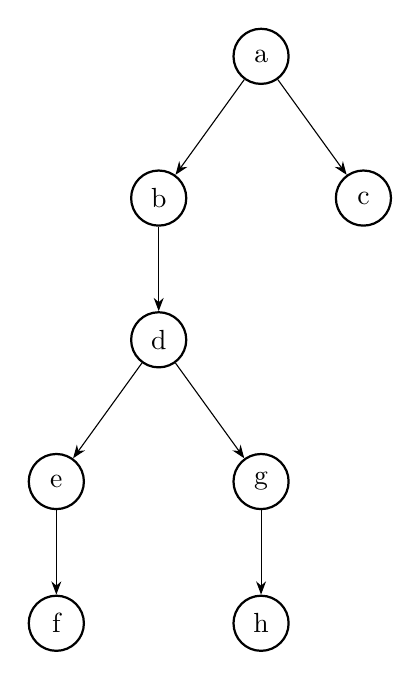
\begin{tikzpicture}[
  level distance=1.8cm,
  sibling distance=2.6cm,
  every node/.style={circle,thick,draw,minimum size=7mm,align=center},
  edge from parent/.style={draw,-{Stealth}} % <-- nuoli + viiva
]
\node (a) {a}
  child { node (b) {b}
    child { node (d) {d}
      child { node (e) {e}
        child { node (f) {f} }
      }
      child { node (g) {g}
        child { node (h) {h} }
      }
    }
  }
  child { node (c) {c} };
\end{tikzpicture}
\end{center}


\pagebreak
\exercise {6. Kyyhkyslakkaperiaate.}
Kyyhkyslakkaperiaatteen mukaan, kun $k$ kyyhkystä sijoitetaan $n$ kyyhkyslakkaan, missä $n<k$, ainakin yhteen kyyhkyslakkaan tulee enemmän kuin yksi kyyhkynen. Tätä periaatetta voidaan soveltaa monissa matemaattisissa todistuksissa, joissa $k$ alkiota luokitellaan $n$:ään luokkaan: Jos $n<k$, ainakin yhteen luokkaan tulee enemmän kuin yksi alkio.
  
{[Sipser Problem 0.10]}
Osoita, että jos suuntaamattomassa verkossa on ainakin kaksi solmua,
niin siinä on kaksi solmua, joiden aste (naapurien lukumäärä)
on sama.
(Tässä kuten yleensäkin suuntaamattomassa verkossa ei
sallita kaarta solmusta itseensä.)\\



\medskip\noindent
\textbf{Todistus.}
...
\end{document}